\documentclass{article}

\usepackage{amssymb}
\usepackage{amsmath}
\usepackage{amsfonts}
\usepackage{enumitem}
\usepackage{graphicx}
\usepackage{fancyhdr}
\usepackage[top=2cm, bottom=4cm, left=2cm, right=2.1cm]{geometry}
\usepackage[most]{tcolorbox}
\usepackage{titlesec}
\usepackage{ifthen}
\usepackage{pgf,pgffor}
\usepackage{datetime}
\usepackage{forloop}
\usepackage{tikz}
\usepackage{booktabs}
\usepackage{pgfplots}
\usetikzlibrary{calc} 
\usetikzlibrary{positioning, arrows.meta}
\pgfplotsset{compat=newest}
\usetikzlibrary{intersections}
\usepgfplotslibrary{fillbetween} 
\usepackage{mdframed}
\usepackage[table]{xcolor}
\usepackage{circuitikz}
\usepackage{mhchem}
% \usepackage{siunitx}
\usepackage[detect-all]{siunitx}

% ----------------------------------------------------
% NEW: two-pass counting
\usepackage{totcount}  
\newtotcounter{totalmarks}
\regtotcounter{totalmarks}
% ----------------------------------------------------

\definecolor{darkerpastelblue}{RGB}{100,149,237}
\definecolor{pastelorange}{RGB}{255,179,71}
\definecolor{lighterpastelblue}{RGB}{100,149,237}
\definecolor{evenLighterBlue}{RGB}{100,149,237}
\definecolor{evenevenLighterBlue}{RGB}{180,209,255}
\definecolor{darkerorange}{RGB}{224, 112, 10}

% Title Format
\titleformat{\section}
{\normalfont\Large\bfseries\color{evenLighterBlue}} 
{} 
{0em} 
{} 
[\titlerule] 

% Header with Level and Subject
\fancyhead[C]{
\includegraphics[height=70pt]{LOGO_GLOW.png}}   
\fancyhead[L]{\LARGE\textcolor{black}{Ganes Assess}} 
\fancyhead[R]{\LARGE\textcolor{darkerpastelblue}{GCSE Mathematics}}  % Dynamic Level and Subject

\pagestyle{fancy}
\lfoot{\textcolor{black}{© \the\year\ Ganes Teaches. All rights reserved.}}
\cfoot{\textbf{\thepage}}
\rfoot{\textcolor{black}{www.ganesteaches.com}}
\setlength{\footskip}{30pt}

\setlength{\headheight}{70pt} 
\renewcommand{\headrulewidth}{2pt} 
\renewcommand{\headrule}{\hbox to\headwidth{\color{pastelorange}\leaders\hrule height \headrulewidth\hfill}}
\renewcommand{\footrulewidth}{0.4pt}
\renewcommand{\footrule}{\hbox to\headwidth{\color{pastelorange}\leaders\hrule height \footrulewidth\hfill}}

\newcounter{loopcntr}

\newcommand{\answerlines}[1]{
    \forloop{loopcntr}{0}{\value{loopcntr}<#1}{
        \textcolor{gray}{\underline{\hspace{\linewidth}}}\\[1ex]
    }
}

% The 'mybox' environment for typed answers
\newtcolorbox{mybox}[2]{
    colback=white,
    colframe=white,
    overlay={
        \node[align=right, text=pastelorange, above=2mm] at (frame.south east) {#2 marks};
    },
    height=#1, % Dynamic height
    boxrule=0pt,
    boxsep=0pt
}

\usepackage{helvet}
\renewcommand{\familydefault}{\sfdefault}

% The environment for each question's marks display
\newtcolorbox{roundedmarksbox}[1][]{ 
    colback=white,               % Background color
    colframe=darkerpastelblue,   % Border color
    arc=6pt,                     % Rounding of corners
    boxrule=0.6mm,               % Thickness of the border
    halign=flush right,          % Align content to the right
    valign=center,               % Vertical alignment
    width=3.2cm,                 % Width of the box
    height=1.0cm,                % Height of the box
    boxsep=2pt,                  % Inner padding
    before=\flushright,          % Automatically right-align content
    after=\hspace{0mm},          % Keep spacing consistent
    #1
}

% ----------------------------------------------------
% Use the same counter for question marks, but let totcount track it
% ----------------------------------------------------
\newcommand{\addmarks}[1]{%
    \addtocounter{totalmarks}{#1}%
}

% A helper macro to place a box with a given number of marks
\newcommand{\QuestionMarks}[1]{%
    % Add to total
    \addmarks{#1}%
    % Print a right-aligned box for the question's marks
    \begin{flushright}
        \begin{roundedmarksbox}
            \textbf{\color{darkerorange}$\ldots$/ #1 mark\ifnum#1>1 s\fi}
        \end{roundedmarksbox}
    \end{flushright}
}

% Define a custom command for a rounded checkbox
\newcommand{\checkbox}{\tikz \node[draw, thick, minimum width=4mm, minimum height=4mm, rounded corners=1mm] {};}

\begin{document}

% Re-style section titles for the main body:
\titleformat{\section}
{\normalfont\Large\bfseries\color{darkerpastelblue}} 
{} 
{0em} 
{} 
[\titlerule] 

% ----------------------------------------
% Front-page tcolorbox
% We show total marks using \total{totalmarks} 
% (requires 2 compilation passes to update)
% ----------------------------------------
\begin{tcolorbox}[
    colback=white!5!white, 
    colframe=pastelorange, 
    title=\LARGE\centering {Vectors - Scale Factors},
    enhanced,
    overlay={
        % Show "Total Marks: ... / <counter>" in bottom-right corner
        \node[anchor=south east, xshift=-5mm, yshift=5mm, text=darkerpastelblue, font=\bfseries] 
        at (frame.south east) {Total Marks: $\ldots$/\total{totalmarks}};
    }
]
\begin{enumerate}

\item \textbf{Position Vectors and Geometry:}
\begin{itemize}
    \item \textcolor{darkerpastelblue}{Key Concept:}
        - A position vector describes the location of a point relative to the origin.
        - Use vectors like \( \vec{AB} = \vec{b} - \vec{a} \) where \( \vec{a} = \vec{OA} \), \( \vec{b} = \vec{OB} \).
        - Midpoint of \( AB \) is \( \frac{1}{2}(\vec{a} + \vec{b}) \).
\end{itemize}

\item \textbf{Collinearity and Straight Lines:}
\begin{itemize}
    \item \textcolor{darkerpastelblue}{Strategy:}
        - Points \( A \), \( B \), \( C \) are collinear if \( \vec{AC} = k\vec{AB} \) for some scalar \( k \).
        - Show one vector is a scalar multiple of another.
\end{itemize}

\item \textbf{Vectors in Triangles:}
\begin{itemize}
    \item \textcolor{darkerpastelblue}{Observation:}
        - Use \( \vec{AB} + \vec{BC} = \vec{AC} \).
        - Triangle formed when 3 vectors connect in a closed loop (resultant = 0).
\end{itemize}

\end{enumerate}







\begin{center}
  \includegraphics[height=100pt]{qrcode_new.png}
  \vspace{2mm}
\end{center}

\end{tcolorbox}






% ---------------- Day 1 ----------------
\newpage
\section*{Day 1}
\vspace{5mm}

\begin{enumerate}


\begin{minipage}[t]{\linewidth}
\item Round I – Use the notes as you work through the question. Given:
\begin{itemize}
  \item $OAC$, $OMB$, and $MDC$ are straight lines.
  \item \( \vec{AC} = 4\vec{OA} \)
  \item \( M \) is the midpoint of \( OB \)
  \item \( \vec{OA} = \vec{2a} \), \( \vec{OB} = \vec{2b} \)
  \item \( \vec{AD} = \lambda \vec{AB} \), where \( \lambda \) is a scalar. Find the value of \( \lambda \).
\end{itemize}

\QuestionMarks{5}

            \begin{center}
            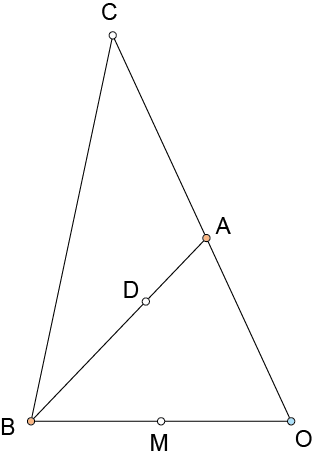
\includegraphics[width=0.45\textwidth]{images/gcse/mathematics/vectors/1.png} 
            \end{center}

\begin{mybox}{35mm}{14}
\answerlines{6}
\end{mybox}
\end{minipage}

\begin{minipage}[t]{\linewidth}
\begin{mybox}{140mm}{14}
\answerlines{32}
\end{mybox}
\end{minipage}


\end{enumerate}


% ---------------- Day 2 ----------------
\newpage
\section*{Day 2}
\vspace{5mm}

\begin{enumerate}

\begin{minipage}[t]{\linewidth}
\item Round II – Review the notes first, then try the question without them. Given:
\begin{itemize}
  \item $OAC$, $OMB$, and $MDC$ are straight lines.
  \item \( \vec{AC} = 4\vec{OA} \)
  \item \( M \) is the midpoint of \( OB \)
  \item \( \vec{OA} = \vec{2a} \), \( \vec{OB} = \vec{2b} \)
  \item \( \vec{AD} = \lambda \vec{AB} \), where \( \lambda \) is a scalar. Find the value of \( \lambda \).
\end{itemize}

\QuestionMarks{5}

            \begin{center}
            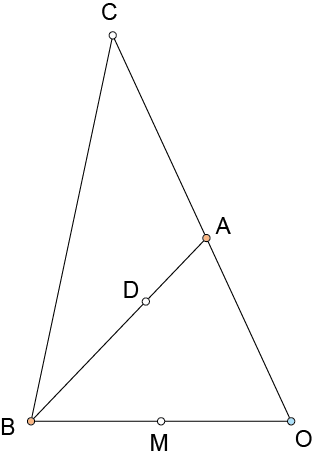
\includegraphics[width=0.45\textwidth]{images/gcse/mathematics/vectors/1.png} 
            \end{center}

\begin{mybox}{35mm}{14}
\answerlines{6}
\end{mybox}
\end{minipage}

\begin{minipage}[t]{\linewidth}
\begin{mybox}{140mm}{14}
\answerlines{32}
\end{mybox}
\end{minipage}

\end{enumerate}


% ---------------- Day 3 ----------------
\newpage
\section*{Day 3}
\vspace{5mm}

\begin{enumerate}

\begin{minipage}[t]{\linewidth}
\item Round III – Attempt the question with no notes at all.
\begin{itemize}
  \item $OAC$, $OMB$, and $MDC$ are straight lines.
  \item \( \vec{AC} = 4\vec{OA} \)
  \item \( M \) is the midpoint of \( OB \)
  \item \( \vec{OA} = \vec{2a} \), \( \vec{OB} = \vec{2b} \)
  \item \( \vec{AD} = \lambda \vec{AB} \), where \( \lambda \) is a scalar. Find the value of \( \lambda \).
\end{itemize}

\QuestionMarks{5}

            \begin{center}
            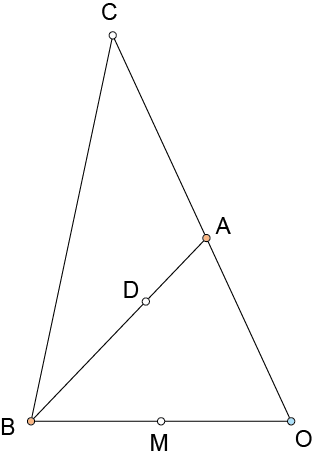
\includegraphics[width=0.45\textwidth]{images/gcse/mathematics/vectors/1.png} 
            \end{center}

\begin{mybox}{35mm}{14}
\answerlines{6}
\end{mybox}
\end{minipage}

\begin{minipage}[t]{\linewidth}
\begin{mybox}{140mm}{14}
\answerlines{32}
\end{mybox}
\end{minipage}

\end{enumerate}


% ---------------- Day 4 ----------------
\newpage
\section*{Day 4}
\vspace{5mm}

\begin{enumerate}

\begin{minipage}[t]{\linewidth}
\item Given:
\begin{itemize}
  \item $ACB$ and $MCO$ are straight lines.
  \item \( M \) is the midpoint of \( DB \)
  \item \( OC:CM \) is in the ratio of \( 3:1 \)
  \item \( \vec{OD} = \vec{2a} \), \( \vec{OB} = \vec{3b} \)
  \item \( \vec{OA} = \mu \vec{OD} \), where \( \mu \) is a scalar. Work out the ratio of OA:AD.
\end{itemize}

\QuestionMarks{5}

            \begin{center}
            \includegraphics[width=0.55\textwidth]{images/gcse/mathematics/vectors/2.png} 
            \end{center}

\begin{mybox}{35mm}{14}
\answerlines{6}
\end{mybox}
\end{minipage}

\begin{minipage}[t]{\linewidth}
\begin{mybox}{140mm}{14}
\answerlines{32}
\end{mybox}
\end{minipage}

\end{enumerate}


% % ---------------- Day 5 ----------------
% \newpage
% \section*{Day 5}
% \vspace{5mm}

% \begin{enumerate}



% \end{enumerate}

\end{document}
